\documentclass[10pt]{article}

\usepackage{spheric}
%%%TITLE
\title{DualSPHysics: a numerical tool to simulate real breakwaters}
\date{}



%%AFFILIATIONS
\author[1]{Feng ZHANG$^\dagger$}
\author[1]{Shaoping SHANG} 
\affil[1]{Xiamen University, China}

\author[2]{Alejandro CRESPO}
\author[2]{Jos\'{e} DOM\'{I}NGUEZ}
\author[2]{Moncho G\'{O}MEZ-GESTEIRA}
\affil[2]{Universidade de Vigo, Spain}

\author[3]{Corrado ALTOMARE}
\affil[3]{Flanders Hydraulic Research \& Ghent University, Belgium}

\author[4]{Andrea MARZEDDU}
\affil[4]{Universitat Polit\`{e}cnica de Catalunya, Spain}

\affil[$\relax$]{\email{\dagger}{zhangfeng@stu.xmu.edu.cn}}


%%DOCUMENT
\begin{document}
\maketitle

%\SelectedTopics{}

%%PLEASE PUT YOUR ABSTRACT HERE
\begin{abstract}
DualSPHysics \cite{crespo2015dualsphysics} is an SPH-based model conceived to be an efficient and user-friendly numerical technique for a wide range of application in the field of hydraulic, naval and coastal engineering. The model is open source and can be freely downloaded from \url{http://www.dual.sphysics.org}. Thanks to the power of GPUs (graphics cards with powerful parallel computing), real engineering problems can be simulated with DualSPHysics using high resolution at a reasonable time. When applied to coastal engineering, the model has been demonstrated to accurately reproduce wave propagation and transformation and wave-structure interaction phenomena. The code is devised to mimic an experimental facility (wave flume or wave basin) and therefore implements automatic wave generation and integrated active wave absorption (AWAS) techniques \cite{altomare2017long}. Moving boundaries are used to mimic the displacement of the wavemaker used in a physical facility. In the present study, a piston-type wavemaker that moves with a pre-imposed displacement is considered to generate regular wave trains.  
The main objectives of the work are:
\begin{enumerate}
\item To validate DualSPHysics in terms of wave run-up on a breakwater with a two layer cubic blocks armor. The numerical results are compared with experimental data of a smooth dike (Figure \ref{fig:22-1}) and a dike with 2 layers of cubic blocks (Figure \ref{fig:22-2}).
\item To apply the validated SPH model to study the run-up on a dike using the real dimensions, bathymetry and waves conditions from the coast of Chongwu (China).
\end{enumerate}

\begin{figure}[!htb]
\begin{minipage}[b]{0.46\linewidth}
\centering
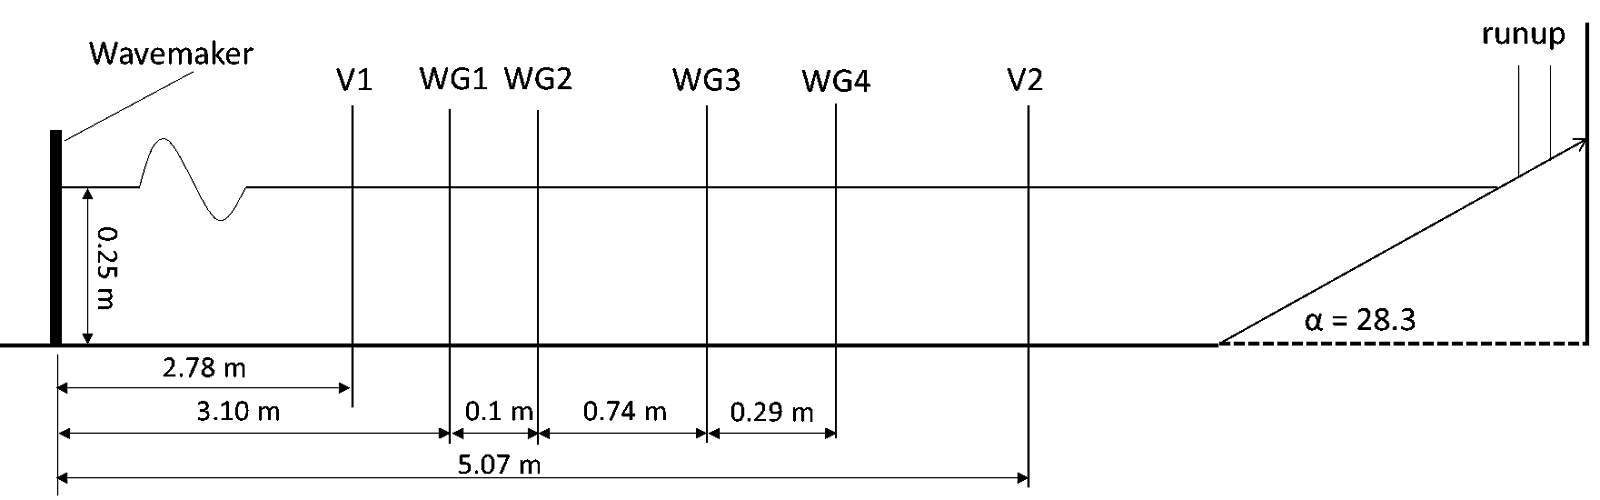
\includegraphics[width=0.96\textwidth]{22-11.png}\\
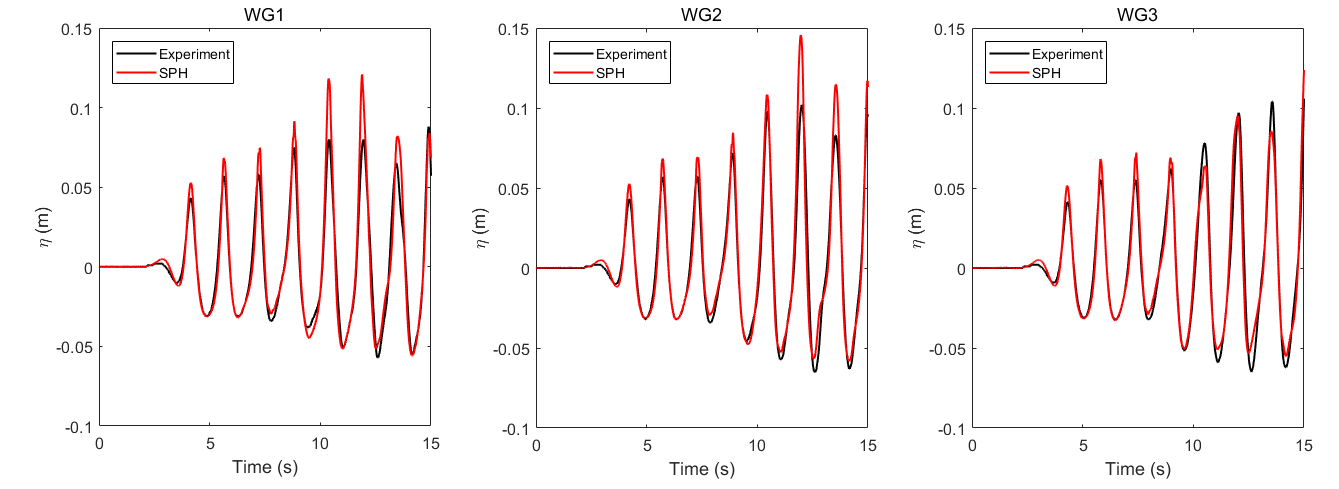
\includegraphics[width=\textwidth]{22-12.png}
\end{minipage}
\begin{minipage}[b]{0.05\linewidth}
~
\end{minipage}
\begin{minipage}[b]{0.46\linewidth}
\centering
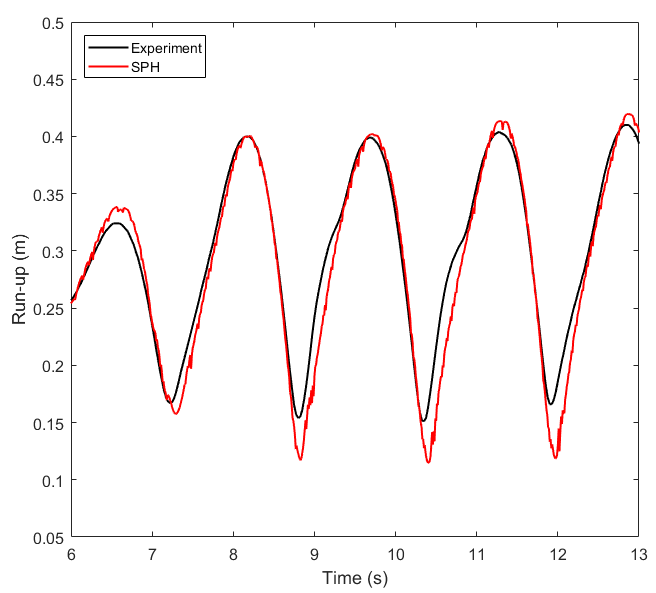
\includegraphics[width=0.8\textwidth]{22-13.png}
\end{minipage}
\caption{Validation of DualSPHysics comparing with experiments of the smooth dike and waves of $H=0.1$ m, $T=1.56$ s, $d=0.25$ m.}\label{fig:22-1}
\end{figure}

\begin{figure}[!htb]
\begin{minipage}[c]{0.37\linewidth}
\centering
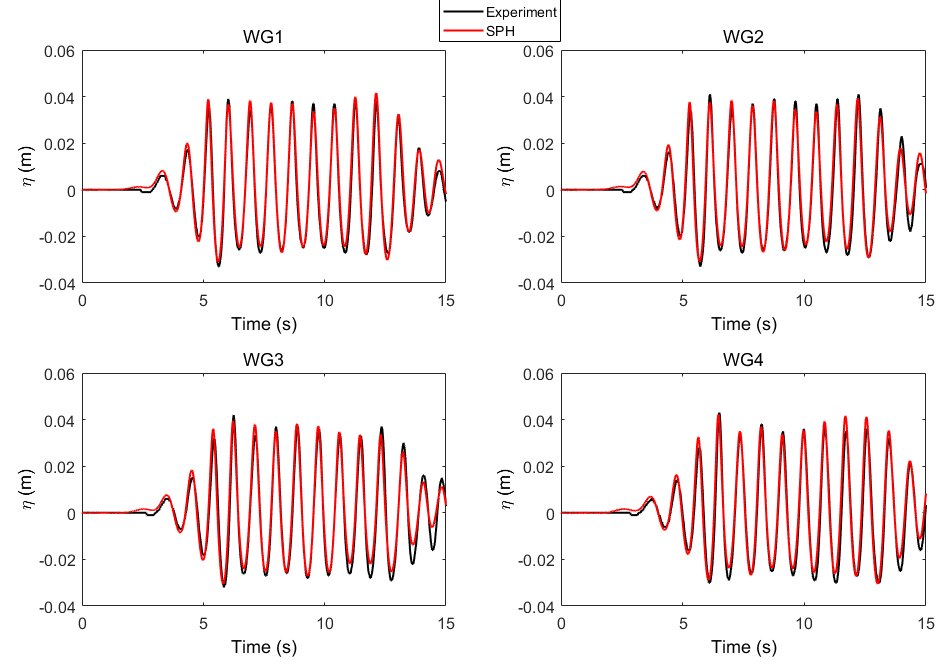
\includegraphics[width=0.95\textwidth]{22-21.png}
\end{minipage}
\begin{minipage}[c]{0.31\linewidth}
\centering
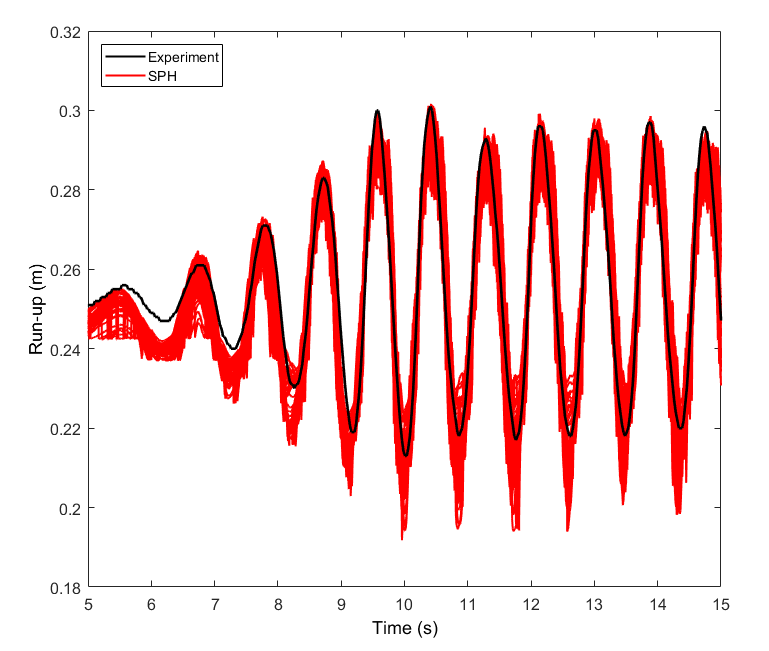
\includegraphics[width=0.95\textwidth]{22-22.png}
\end{minipage}
\begin{minipage}[c]{0.31\linewidth}
\centering
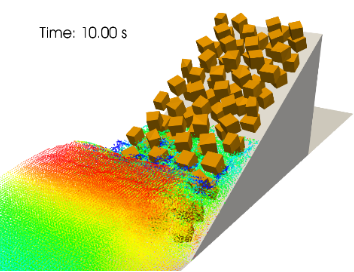
\includegraphics[width=0.95\textwidth]{22-23.png}
\end{minipage}
\caption{Validation of DualSPHysics comparing with experiments of the breakwater with a two layer cubic blocks armor and waves of $H=0.08$ m, $T=0.87$ s, $d=0.25$ m.}\label{fig:22-2}
\end{figure}

As first \textbf{novelty}, a proper validation of run-up is here performed since we have compared the numerical and experimental time series of water surface elevation and time series of wave run-up. Previous work \cite{altomare2014numerical} presented a validation for run-up, but only a maximum value for different incoming waves was compared with experimental and literature data. The time series of the experimental wavemaker is assigned to the numerical one. Figure \ref{fig:22-1} and \ref{fig:22-2} shows the result of the validation with experiments using the smooth and the porous dike, respectively. Note that run-up for the armor block dike is numerically computed at 52 different positions along the width of the channel to catch the three-dimensional behavior. Several different wave conditions are simulated and overall \textbf{good accuracy} is obtained for both wave surface elevation and time series of the run-up.

The second \textbf{novelty} is the application of the SPH model to a real problem using the dimensions of a dike in China. In this case wave conditions are imposed based on real wave condition in situ and AWAS \cite{altomare2017long} is employed to compensate the wave reflection at the numerical wavemaker. This is mandatory to mimic the real open sea. Therefore, once the model has been properly validated with experiments \textbf{it can be applied to study real situations} in the coast of Chongwu.

\end{abstract}


%%THE END OF ABSTRACT

\addbib

\end{document}
